\documentclass{beamer}
\usepackage{beamerthemesplit}
\usepackage{wrapfig}
\usetheme{SPbGU}
\usepackage{pdfpages}
\usepackage{amsmath}
\usepackage{cmap} 
\usepackage[T2A]{fontenc} 
\usepackage[utf8]{inputenc}
\usepackage[english,russian]{babel}
\usepackage{indentfirst}
\usepackage{amsmath}
\usepackage{tikz}
\usepackage{array}
\usepackage{multirow}
\usepackage[noend]{algpseudocode}
\usepackage{algorithm}
\usepackage{algorithmicx}
\usepackage[absolute,overlay]{textpos}
\usetikzlibrary{shapes,arrows}
\usepackage{fancyvrb}
\newtheorem{rutheorem}{Теорема}
\newtheorem{ruproof}{Доказательство}
\newtheorem{rudefinition}{Определение}
\newtheorem{rulemma}{Лемма}
\beamertemplatenavigationsymbolsempty

\title[]{Оптимизация алгоритма лексического анализа 
динамически формируемого кода}
% То, что в квадратных скобках, отображается в левом нижнем углу. 
\institute[СПбГУ]{
Санкт-Петербургский государственный университет \\
Кафедра системного программирования }

% То, что в квадратных скобках, отображается в левом нижнем углу.
\author[Александр Байгельдин]{Александр Байгельдин, студент СПбГУ\\
  % У научного руководителя должна быть указана научная степень
  \and  
    {\bfseriesНаучный руководитель:} ст.пр., магистр ИТ С.В. Григорьев}

\date{18 мая 2016г.}

\definecolor{orange}{RGB}{179,36,31}

\begin{document}
{
% Лого университета или организации, отображается в шапке титульного листа
\begin{frame}
  \begin{center}
  {
\includegraphics[width=1.5cm]{pictures/SPbGU_Logo.png}}
  \end{center}
  \titlepage
\end{frame}
}

\begin{frame}[fragile]
  \transwipe[direction=90]
  \frametitle{Динамически формируемый код}
  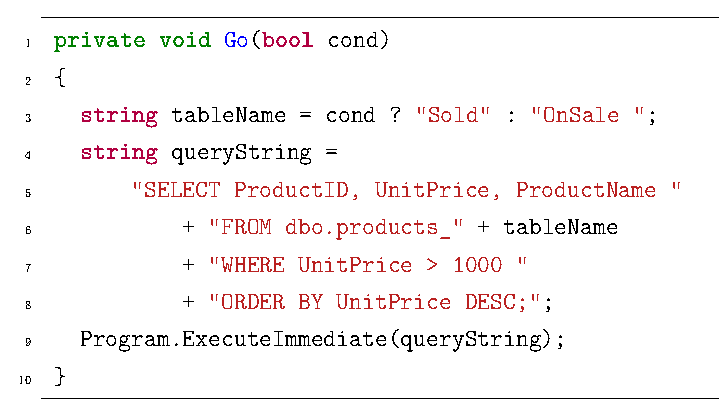
\includegraphics[width=11cm]{pictures/intro_code.pdf}
\end{frame}
            
\begin{frame}[fragile]
  \transwipe[direction=90]
  \frametitle{Лексический анализ}
  В классическом лексическом анализе применяются конечные преобразователи 
  (Finite State Transducers) \\[1\baselineskip]
  \footnotesize
  \begin{Verbatim}[commandchars=\\\{\}]
      rule token = parse
      | [\textcolor{red}{'0'}-\textcolor{red}{'9'}]  \{ \textcolor{green}{Some}(\textcolor{blue}{NUM}(gr)) \}
      | \textcolor{red}{'+'}  \{ \textcolor{green}{Some}(\textcolor{blue}{PLUS}(gr)) \}
  \end{Verbatim}
  \normalsize
  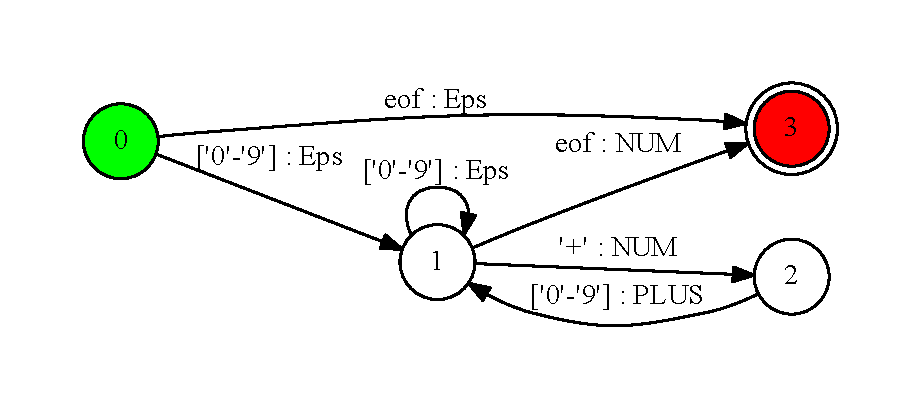
\includegraphics[width=9cm]{pictures/lexer_.pdf}
\end{frame}

\begin{frame}
  \transwipe[direction=90]
  \frametitle{Регулярная аппроксимация}
  Для динамически формируемого кода можно построить регулярную 
  аппроксимацию \\[2\baselineskip]
  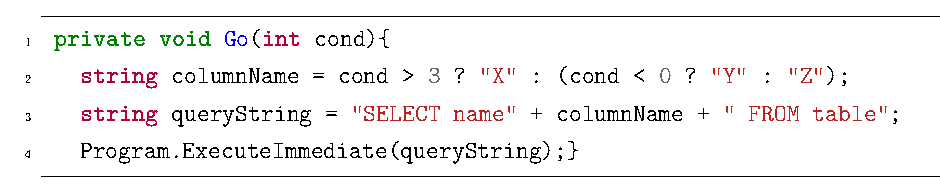
\includegraphics[width=11cm]{pictures/approx_code.pdf} \\
  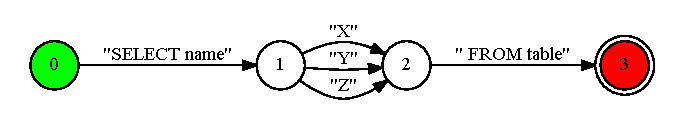
\includegraphics[width=11cm]{pictures/approx_fsa.pdf}
\end{frame}

\begin{frame}
  \transwipe[direction=90]
  \frametitle{Композиция FST}
  \begin{textblock}{12}(0.5, 3)
    Важной частью лексического анализа динамически формируемого
    кода является операция композиции FST (\textbf{T = T1 $\circ$ T2})
  \end{textblock}
  \begin{textblock}{12}(0.3, 6.8)
    \textbf{T1}
  \end{textblock}
  \begin{textblock}{12}(0.5, 5)
    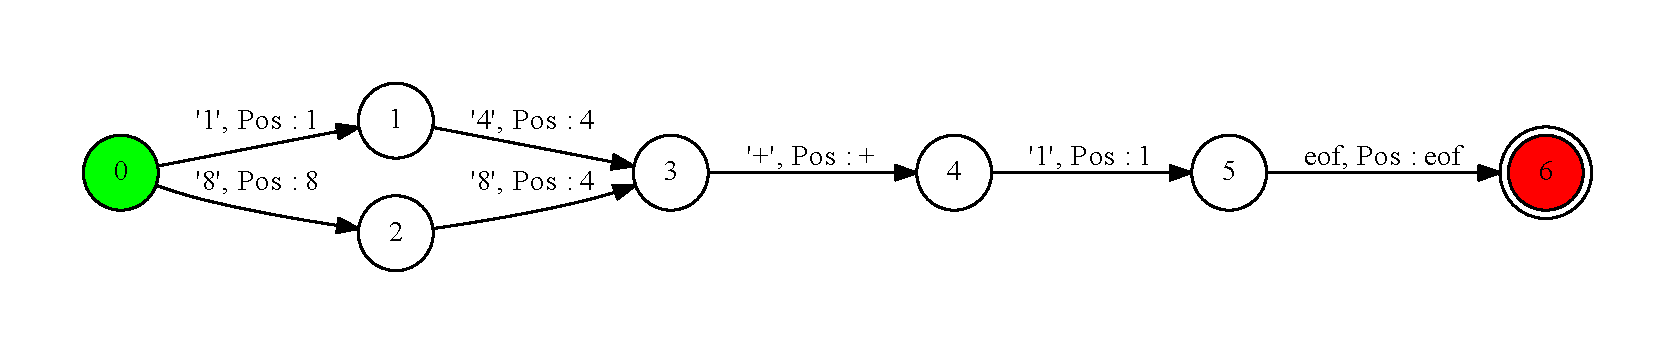
\includegraphics[width=12cm]{pictures/example_.pdf}
  \end{textblock}
  \begin{textblock}{12}(0.3, 9.2)
    \textbf{T2}
  \end{textblock}
  \begin{textblock}{8}(0.3, 7.5)
    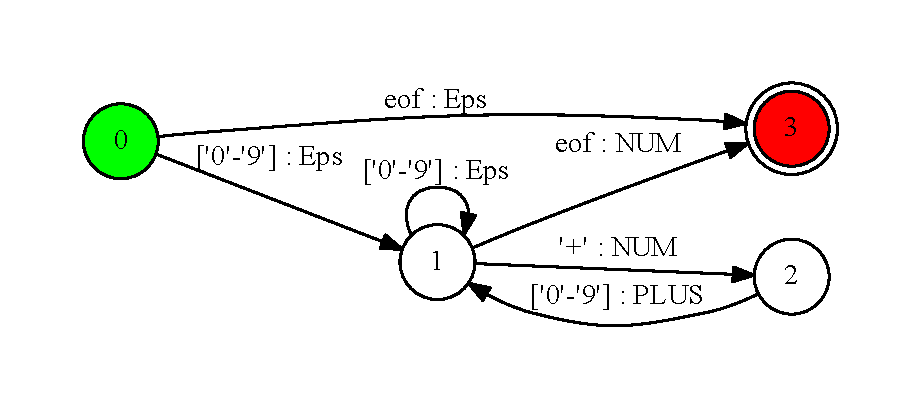
\includegraphics[width=8cm]{pictures/lexer_.pdf}
  \end{textblock}
  \begin{textblock}{12}(0.4, 13.5)
    \textbf{T}
  \end{textblock}
  \begin{textblock}{12}(0.5, 12)
    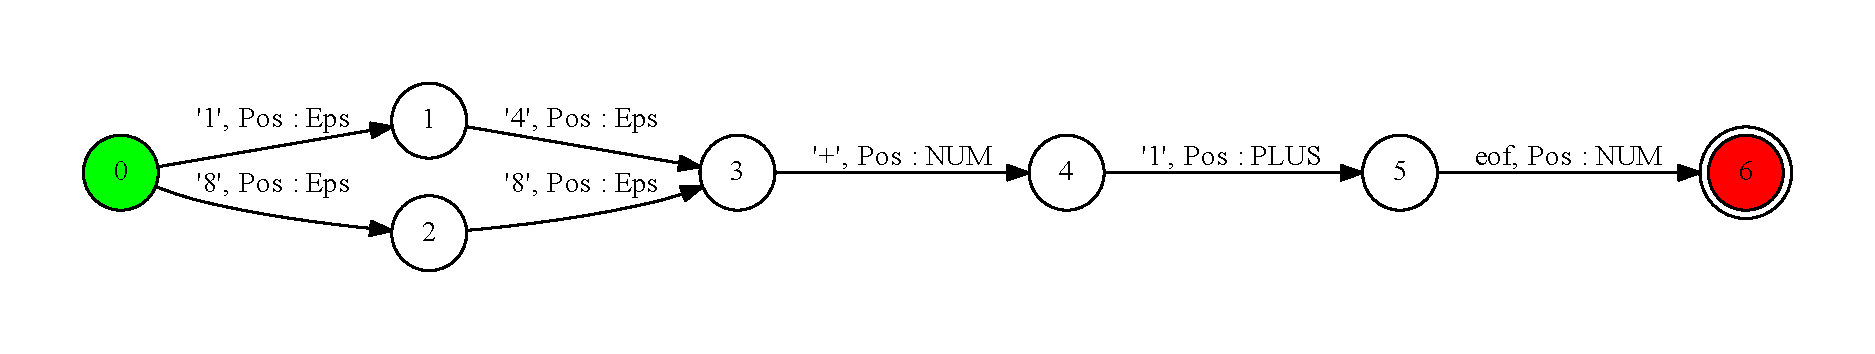
\includegraphics[width=12cm]{pictures/res_.pdf}
  \end{textblock}
\end{frame}

\begin{frame}
  \transwipe[direction=90]
  \frametitle{YaccConstructor}
  \begin{itemize}
    \item YaccConstructor — исследовательский проект в области 
    лексического и синтаксического анализа
    \item В YaccConstuctor для лексического анализа динамически формируемого кода
    применяется подход, в основе которого лежит построение  регулярной аппроксимации и 
    композиция FST
    \item Реализованный в YaccConstructor алгоритм композиции FST обладает недостаточной
    производительностью
  \end{itemize}
\end{frame}

% Обязательный слайд: четкая формулировка цели данной работы и постановка задачи
% Описание выносимых на защиту результатов, процесса или особенностей их достижения и т.д.
\begin{frame}
  \transwipe[direction=90]
  \frametitle{Постановка задачи}
  \textbf{Целью} работы является исследование возможности улучшения
  производительности лексического анализа динамически 
  формируемого кода\\[2\baselineskip]

  \textbf{Задачи}:
  \begin{itemize}
    \item Исследовать алгоритмы композиции FST
    \item Реализовать и интегрировать в проект YaccConstructor более оптимальный алгоритм композиции
    \item Сравнить производительность реализаций текущего и выбранного алгоритмов
  \end{itemize}
\end{frame}

\begin{frame}
  \transwipe[direction=90]
  \frametitle{Решение}
  \begin{itemize}
    \item Временная сложность текущего алгоритма: \\
    \[O(V_1 * V_2 * D_1 * D_2)\]
    где V — число вершин, D — максимальное количество исходящих ребер
    \item В текущем алгоритме образуются недостижимые вершины, которые приходится удалять
    \item Временная сложность выбранного алгоритма: \\
    \[O(V_1 * V_2 * D_1 * (log(D_2) + M_2))\]
    где M — степень недетерминированности
    \item В выбранном алгоритме недостижимых вершин не образуется
  \end{itemize}
\end{frame}

\begin{frame}
  \transwipe[direction=90]
  \frametitle{Особенности реализации}
  \begin{itemize}
    \item F\# — язык семейства .NET
    \item YaccConstructor — исследовательский проект в области лексического и синтаксического анализа
    \item QuickGraph — библиотека .NET для работы с графами
    \item Реорганизация проекта YaccConstructor
    \begin{itemize}
      \item Библиотека для работы с конечными преобразователями YC.FST интегрирована в проект QuickGraph
      \item Произведен рефакторинг, заключавшийся в подмене сторонней библиотеки QuickGraph в YaccConstructor на использование собственной сборки
    \end{itemize}
  \end{itemize}
\end{frame}

\begin{frame}
  \transwipe[direction=90]
  \frametitle{Измерения}
    \begin{center}
        \begin{tabular}{ | p{1.5cm} | p{1.5cm} | p{3.2cm} | p{3.4cm} | }
        \hline
        Кол-во вершин & Кол-во ребер & 
        Время работы текущего алгоритма (мс) & 
        Время работы выбранного алгоритма (мс) \\ \hline
        250 & 738 & 16526 & 1133 \\ \hline
        711 & 1766 & 30285 & 2068 \\ \hline
        215 & 895 & 4045 & 248 \\ \hline
        310 & 687 & 7184 & 394 \\ \hline
        \end{tabular}
    \end{center}
    Математическое ожидание и среднее квадратичное отклонение ускорения (в кол-ве раз) выбранного алгоритма по сравнению с текущим:
    \[M = 18.7, \sigma = 3.23\]
\end{frame}

\begin{frame}
  \transwipe[direction=90]
  \frametitle{Результаты}
  \begin{itemize}
    \item Исследованы алгоритмы композиции FST
    \item Выбранный алгоритм реализован и интегрирован в проект YaccConstructor
    \item Произведено сравнение производительности реализаций текущего и выбранного алгоритмов
    \item Выступление на конференции «Современные технологии в теории и практике программирования»
    \begin{itemize}
      \item Публикация в сборнике конференции
    \end{itemize}
  \end{itemize}
\end{frame}

\end{document}